\StartPlate{V12}{The principal-period filter}{The period belongs to the actual order, and the level must be integral.}
\begin{center}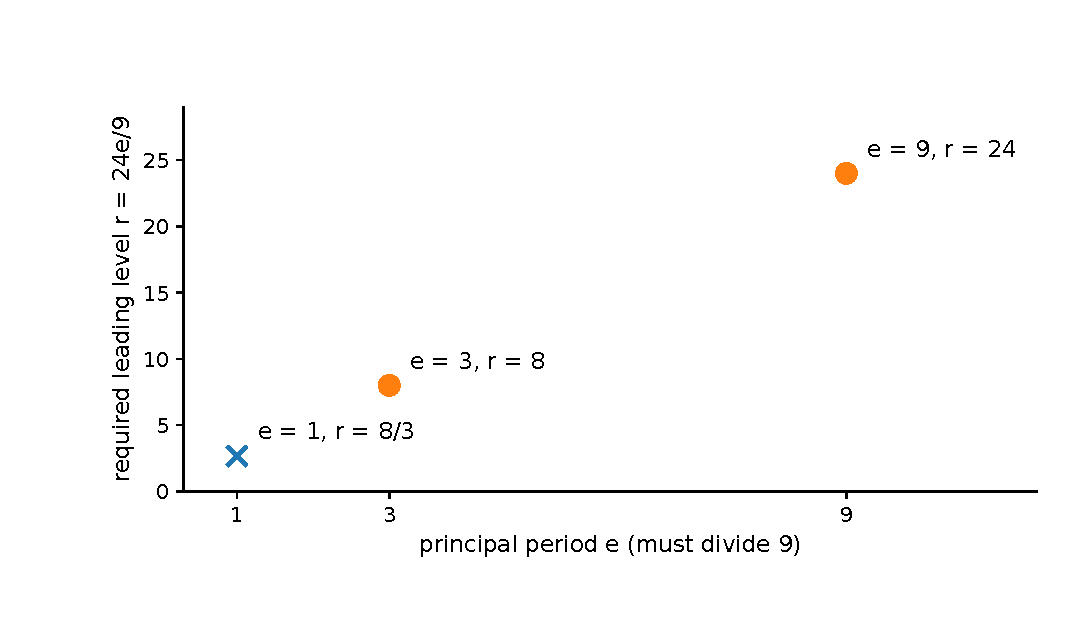
\includegraphics[width=\linewidth]{figures/V12.pdf}\end{center}
Under the stated actual-type conductor formula, a rank-$n$ source with Swan conductor $w$ requires $nr=ew$, where the principal period satisfies $e\mid n$. Therefore
\[
\frac{n}{\gcd(n,w)}\mid e\mid n,
\qquad r=\frac{ew}{n}.
\]
For $(n,w)=(9,24)$, period one would demand the nonintegral level $8/3$. Periods three and nine leave $(e,r)=(3,8)$ and $(9,24)$. The cross is excluded numerically. The circles pass only this integrality condition.

A period-three candidate can still fail the independent torsion-number test when its actual maximal parameter field has residue degree three. The prescribed wild-irreducible source has no nontrivial unramified self twist. Neither a convenient lattice period nor a lower critical level can be substituted for the actual period and leading level in the formula. A necessary numerical pass supplies no simple stratum or character occurrence by itself.
\vfill\PlateSource{Exact necessary filter}{Part III, Section 22.2--22.3}{58}
